\newchap{Data Sets}
\label{chap:5_dataset}

\section{gliGLUE}


\begin{Verbatim}[commandchars=\\\{\}]
Ich        B-A0         O
fühlte     \colorbox{blue}{B-V}          O
[MASK]     B-A1         O
,          I-A1         O
als        I-A1         O
ich        I-A1         \textit{B-A0}
aus        I-A1         \textbf{O}
Versehen   I-A1         O
schlechte  I-A1         B-A1
Milch      I-A1         I-A1
\colorbox{blue}{getrunken  I-A1         \textbf{B-V}}
habe       I-A1         O
\end{Verbatim}


Traditionally in linguistics, language is analyzed into different structural levels, where
different tools for describing these levels, or strata, are used.
In most theories, there are are four of these structural levels proposed:
Beginning from the Bottom, there is the level of Phonetics and Phonology, followed by Morphology,
then there is the level of Syntax, and the last one is Semantics.\myfootnote{Sometimes Pragmatics
is conceptualized as an additional fifth layer on top, sometimes it is considered to form a field
of its own; I follow the latter.}
While the first three levels deal with the form of utterances of human language, semantics is
concerned with the meaning of such utterances \citep[p.~4ff.]{kracht2007introduction}.

% \tab{tab:levels-of-lang}{Levels of language analysis and description.}
% {\begin{tabular}{|l|l|l|l|}
% \hline
% \multicolumn{2}{|c|}{Form}     & \multicolumn{2}{c|}{Meaning}     \\ \hline
%   % a & b & c & d \\ \hline
%   & \multicolumn{2}{c|}{Level} &                   \\ \hhline{====}
%         Syntax  & \multicolumn{2}{l|}{Sentence} & \multirow{3}{*}{Semantics} \\ \cline{1-3}
%         Morphology & \multicolumn{2}{l|}{Word} &                   \\ \cline{1-3}
%         Phonology & \multicolumn{2}{l|}{Sound} &                   \\ \hline
% \end{tabular}
% }{Levels of language}


Following \cite{wang2018glue},

\tab{tab:original-GLUE}{Original GLUE data sets and tasks (following the table from \cite{wang2018glue}).}{
  \resizebox{\textwidth}{!}{
    \begin{tabular}{l|llll}
      Data Set & NLP Task                   & ML Task                    & \# Examples & Splits \\ \hline\hline
      & \multicolumn{4}{c}{\textit{Single-Sentence Tasks}} \\
      CoLA     &  Acceptability             & Binary Classification      & 8.5k/1k & train/test \\
      SST-2    & Sentiment Analysis         & Binary Classification      & 67k/1.8k & train/test \\
      \hline
      & \multicolumn{4}{c}{\textit{Sentence Pair Tasks}} \\
      MNLI     & Natural Language Inference & Multi-Class Classification &  393k/20k & train/test \\
      MRPC     & Paraphrase Identification  & Binary Classification      & 3.7k/1.7k & train/test \\
      QNLI     & Question Answering         & Binary Classification\myfootnote{\cite{wang2018glue} reformulate the original SQuAD task CITE of predicting an answer span in the context into a sentence pair binary classification task: They pair each sentence in the context with the question and predict whether or not the context sentence includes the answer span.} &  105k/5.4k & train/test \\
      QQP      & Paraphrase Identification  & Binary Classification      &  364k/391k & train/test \\
      RTE      & Natural Language Inference & Binary Classification\myfootnote{\cite{wang2018glue} combine several data sets into RTE; for data sets that have three labels --- \emph{entailment}, \emph{neutral}, and \emph{contradiction} --- they collapse the latter two into one label \emph{not\_entailment}.} &  2.5k/3k & train/test \\
      STS-B    & Sentence Similarity        & Regression (1 - 5)         & 7k/1.4k & train/test \\
      WNLI     & Coreference Resolution     & Binary Classification\myfootnote{In the original Winograd Schema Challenge CITE, the task is to choose the correct referent of a pronoun from a list. \cite{wang2018glue} reformulate this to a sentence pair classification task, where the original sentence is paired with the original sentence with each pronoun substituted from the list and then predicting whether the substituted sentence is entailed by the original one.} &  634/146 & train/test
    \end{tabular}
  }
}{GLUE}


\tab{tab:overview-data-sets}{gliGLUE data sets and tasks.}{
  \resizebox{\textwidth}{!}{
    \begin{tabular}{l|llll}
      Data Set & NLP Task                   & ML Task                    & \# Examples        & Splits \\ \hline\hline
      & \multicolumn{4}{c}{\textit{Single-Sentence Tasks}} \\
      deISEAR  & Emotion Detection          & Multi-Class Classification & 1 001              & - \\
      SCARE    & Sentiment Analysis         & Multi-Class Classification & 1 760              & - \\
      \hline
      & \multicolumn{4}{c}{\textit{Sentence Pair Tasks}} \\
      % SCARE Reviews &  Sentiment Analysis & Multi-Class Classification & 802 860 & - \\
      MLQA     & Question Answering         & Span Prediction            & 509/4 499          & dev/test \\
      PAWS-X   & Paraphrase Identification  & Binary Classification      & 14 402/2 000/4 000 & train/dev/test \\
      XNLI     & Natural Language Inference & Multi-Class Classification &  2 489/7 498       & dev/test \\
      XQuAD    & Question Answering         & Span Prediction            &  1 192             & -
    \end{tabular}
  }
}{gliGLUE}

\subsection{General Issues}

There are a few remarks and strategies that apply to all collected corpora:

(1) All of the data sets except deISEAR are not monolingual, i.e. German, sources, but bi-
or multilingual corpora. To compile a German GLUE corpus I only use the German subset of
those corpora. For example, the MLQA data set provides all 49 combinations of the languages
it contains: Context in Arabic, question in Hindi; context in English, question in Spanish,
etc. Also in this case, I choose only the German-German part of the data set for my corpus.

(2) The data sets I chose for my little GLUE corpus are being provided in different modes.
While three of the corpora, namely MLQA, PAWS-X, and XNLI, come with a predefined split, the
others are made available without splits.
In the latter case, I split the data sets into train, development, and test splits using a 0.7,
0.15, and 0.15 portion, respectively.
Interestingly, the data sets that come with splits, only provide a development and test portion.
To ensure that my results are comparable with those that the authors of the different data sets
report, I leave the test split as it is, and split the development set into a train and
development set, implementing a 85:15 ratio.

(3) Most of the data sets were constructud by translating existing monolingual English
data sets (semi-)automatically into the different target languages. As I show in section
{\color{red} REFXXXX}, this does not come without introducing noise into the data.

The following differences to the original GLUE corpus must be noted:

(1) While \cite{wang2018glue} reformulate a multitude of tasks into inference tasks, I follow in
my implementation \cite{zhang2019semantics} and approach the question answering tasks as
\cite{devlin2018bert} in the original BERT implementation; i.e. as span prediction task.

(2) I tried to combine a multitude of different tasks into my GLUE dataset (single sentence tasks
vs bi- or multiple sentence tasks, classification vs. span detection, different semantic problems
such as emotion detection, question answering etc.), I could not compile all tasks that appear in
GLUE into my semantic dataset compilation.
For example, there are data sets that concern linguistic acceptability in the original GLUE
corpus, such as  e.g. CoLA \cite{warstadt2019neural}, or XXX .
To disregard this task was not an intentional decision, but due to fact that there are simply not
as many datasets available for German and apparently there are no datasets addressing linguistic
acceptability in German.

\section{Corpora}

In this section, I give a detailed description of the selected data sets in alphabetical order:
What kind of task is addressed, what is the text variety, how looks the label distribution, etc.

\subsection{deISEAR}

\subsubsection{Task}

This data set addresses the task of Emotion recognition, a sub-task of Sentiment Analysis.
Technically, it is a sequence classification problem: Given a sequence of tokens, predict the
correct label from a fixed set of emotions.
Following by the original study ``International Survey on Emotion Antecedents and Reactions''
\citep{scherer1994evidence}, \cite{troiano2019crowdsourcing} constructed their data set for German:
In a first step, the authors presented annotators with one of seven emotions, and asked them to
come up with a textual description of an event in which they felt that emotion.
The task was formulated as a sentence completion, so the annotators, which were recruited via an
crowdsourcing platform, had to complete sentences having the following structure: ``Ich fühlte
\emph{emotion}, als/weil/dass ...''.
Seven emotions were given for which the descriptions had to be constructed:
Traurigkeit, Ekel, Schuld, Wut, Angst, Scham, Freude.
For \emph{Traurigkeit} and \emph{Ekel} there are 144 examples in the data set, for the other
emotions there are 143.

\begin{examples}
  \item Ich fühlte \textbf{[Traurigkeit]}, als mein Laptop kaputt ging und die Garantie schon abgelaufen war.
\end{examples}
\begin{examples}
  \item  Ich fühlte \textbf{[Scham]}, weil mir mal beim Urlaub das Geld ausging.
\end{examples}
\begin{examples}
  \item Ich fühlte \textbf{[Angst]}, als der Chef sagte dass Mitarbeiter gekündigt werden müssen.
\end{examples}
\begin{examples}
  \item Ich fühlte \textbf{[Ekel]}, als ich verschimmeltes Essen im Kühlschrank gefunden habe.
\end{examples}
\begin{examples}
  \item Ich fühlte \textbf{[Schuld]}, dass ich meinen besten Kumpel versetzt habe.
\end{examples}

%The searched emotion is \emph{Traurigkeit} in example \ref{ex:deisear}.

%\fig{images/deISEAR_traindevtest.png}{fig:deISEAR-devtest}{Distribution of emotions in the deISEAR data set.}{15}{deISEAR statistics}

\subsubsection{Statistics}

number of examples: \\
train: 700 \\
dev: 150 \\
test: 151

\textbf{merged} \\
average length train: 15.9 (sigma 6.6) \\
average length dev: 17.9 (sigma 19.9) \\
average length test: 17.1 (sigma 7.4)

\textbf{subtokenized} \\
average length train: 18.1 (sigma 7.9) \\
average length dev: 20.7 (sigma 24.1) \\
average length test: 19.5 (sigma 8.8)

% \fig{images/deISEAR_subtokenized.pdf}{fig:deISEAR-context}{deISEAR: Length of subtokenized Sentences.}{8}{deISEAR-Length}
% \fig{images/deISEAR_subtokenized_all.pdf}{fig:out-deISEAR-context}{deISEAR: Length of subtokenized Sentences (with one extreme outlier).}{8}{deISEAR-Length}

\begin{figure}
  \begin{minipage}{0.45\linewidth}
  \vspace{0pt}
    \includegraphics[width=1.0\linewidth]{images/deISEAR_subtokenized.pdf}
  \end{minipage}
  \hfill
  \begin{minipage}{0.45\linewidth}
  \vspace{0pt}
    \includegraphics[width=1.0\linewidth]{images/deISEAR_label_percentages.pdf}
  \end{minipage}
  \stepcounter{myfigure}
  \caption[XNLI Lengths]{\textbf{Left}: Length of subtokenized deISEAR sentences. Note that one extreme outlier in the
                          development set comprising 300 BERT-subtokens is not included in the plot. \textbf{Right}: Label distributions in deISEAR.}
\end{figure}


\subsubsection{SOTA}

\cite{troiano2019crowdsourcing} train a maximum entropy classifier with L2 regularization with
boolean unigram features on the original ISEAR corpus (7665 instances).
Since the original ISEAR study and data collection was carried out in English, they then machine
translate the 1,001 deISEAR examples and evaluate on them.
Using this strategy, the authors accomplish an average micro F$_1$ of 47. (Note: micro F$_1$ in settings where each example gets
exactly one label assigned is the same as accuracy)

\subsection{MLQA}

\subsubsection{Task}

\begin{examples}
  \label{ex:mlqa}
  \item Rita Sahatçiu Ora (* 26. November 1990 in Priština, SFR Jugoslawien) ist eine britische Sängerin und Schauspielerin kosovarischer Herkunft. Von 2010 bis 2016 stand sie bei Jay Z und Roc Nation unter Vertrag. Seit 2017 steht sie bei Atlantic Records unter Vertrag.
\end{examples}

\begin{enumerate}
  \item Wann wurde Rita Sahatçiu Ora geboren? $\rightarrow$ 26. November 1990
\end{enumerate}

\cite{lewis2019mlqa} compiled

PROBLEM: 231 out of 5,008 exceed tokenized length of 512 $\rightarrow$ ignore? 4.6\%

\subsubsection{Statistics}

number of examples: \\
train: 432 \\
dev: 77 \\
test: 4,499

\textbf{merged} \\
average length train answer: 4.0 (sigma 4.9) \\
average length dev answer: 3.7 (sigma 5.4) \\
average length test answer: 4.0 (sigma 5.1)

average length train question: 9.4 (sigma 3.7) \\
average length dev question: 8.6 (sigma 3.4) \\
average length test question: 9.1 (sigma 3.4)

average length train context: 127.7 (sigma 110.0) \\
average length dev context: 125.1 (sigma 116.7) \\
average length test context: 129.9 (sigma 123.1)

\textbf{subtokenized} \\
average length train answer: 5.6 (sigma 6.6) \\
average length dev answer: 5.2 (sigma 6.7) \\
average length test answer: 5.6 (sigma 7.0)

average length train question: 11.4 (sigma 4.5) \\
average length dev question: 10.6 (sigma 4.3) \\
average length test question: 11.2 (sigma 4.3)

average length train context: 162.7 (sigma 139.0) \\
average length dev context: 159.4 (sigma 145.6) \\
average length test context: 165.5 (sigma 156.7)

\subsubsection{SOTA}

\cite{lewis2019mlqa} train their cross-lingual transfer model on the 100,000 instances of SQuAD
\cite{rajpurkar2016squad} as training data.
They use the English development set of MLQA for tuning.
At test time, the model must extract the answer span in the target language.
They report that XLM performs best for German, achieving a 47.6\% accuracy of exact matches, i.e.
predicting the exact start and end span of the answer.

The total of all instances in all languages in MLQA is 46,444.

\subsection{PAWS-X}

The PAWS-X corpus \cite{yang2019paws} was compiled to provide a multilingual source for training
models that address the problem of paraphrase identification.
Since most corpora for this task are available only in English the authors compiled this corpus by
humanly translate a subset of the original PAWS corpus \cite{zhang2019paws}.

\begin{examples}
  \label{ex:paws-x}
  \item Die Familie zog 1972 nach Camp Hill, wo er die Trinity High School in Harrisburg, Pennsylvania, besuchte.

  1972 zog die Familie nach Camp Hill, wo er die Trinity High School in Harrisburg, Pennsylvania, besuchte.
\end{examples}

The label for the sentence pair \ref{ex:paws-x}, of course, would be \emph{true}, since sentence
one is a paraphrase of sentence two, and vice versa.

% TODO: new stats figure!
%\fig{}{fig:PAWS-X-devtest}{Distribution of paraphrases (True) versus non-paraphrases (False) in the PAWS-X data set.}{15}{PAWS-X statistics}
stats

\subsubsection{Preprocessing}

During the preprocessing of this data set, the following considerations are taken into account:

In the predefined development and test splits, there are some examples where one or both sentences
consist
only of the string ``NS''.
I decided to not include this examples into the data used for training and evaluating my models,
since
those examples don't contribute any useful features for the model.\myfootnote{The authors don't
comment on these obscure sentences, so I do not know what was the reasoning behind including these
into the data sets.}
Further, some examples consist of empty strings; I treat those the same way as the examples
mentioned before.

Further, there are sentences XXXXX

\subsubsection{Statistics}

Since the training data are solely machine-translated while the development and test data are
human-translated, there needs to be some clarification as to how differently those sets are.
One measure to capture similarities between sentences is the BLEU score \cite{papineni2002bleu}:
This score measures the overlap of n-grams between two sentences, such that XXX
The BLEU score is a value between 0 (no n-gram overlaps) to 1 (perfect n-gram overlaps), where a
BLEU score of 1 means that the two sentences are identical. As for other measures, like accuracy
e.g., the value is sometimes multiplied by 100 for better readabilit, which I will also do here.

% \fig{images/PAWS-X_subtokenized_sum_without_outlier.pdf}{fig:paws-x-length}{PAWS-X: Length of subtokenized, concatenated sentence pairs.}{8}{PAWS-X-Length-all}

% \fig{images/PAWS-X_subtokenized_sum.pdf}{fig:out-paws-x-length}{PAWS-X: Length of subtokenized, concatenated sentence pairs (with one extreme outlier).}{8}{PAWS-X-Length}
\begin{figure}
  \begin{minipage}{0.45\linewidth}
  \vspace{0pt}
    \includegraphics[width=1.0\linewidth]{images/PAWS-X_subtokenized_sent1.pdf}
  \end{minipage}
  \hfill
  \begin{minipage}{0.45\linewidth}
  \vspace{0pt}
    \includegraphics[width=1.0\linewidth]{images/PAWS-X_subtokenized_sent2.pdf}
  \end{minipage}
  \stepcounter{myfigure}
  \caption[PAWS-X Lengths]{\textbf{Left}: Length of subtokenized PAWS-X first sentences. \textbf{Right}: Length of subtokenized PAWS-X second sentences..}
\end{figure}

Mean BLEU-scores for sets:

Train: 55.27 stdev: 24.97\\
Development: 37.33 stdev: 25.57\\
Test: 38.37 stdev: 24.83


\fig{images/PAWS-X_BLEU_scores.pdf}{fig:PAWS-X-BLEU}{PAWS-X: BLEU scores of data sets.}{8}{PAWS-X-BLEU}


Number of instances: \\
Train: 48,977 \\
Dev: 1,932 \\
Test: 1,967

\textbf{merged} \\
average lenght sentence 1 train: 21.0 (sigma 6.5) \\
average length sentence 2 train: 21.0 (sigma 5.8)

average length sentence 1 dev: 21.1 (sigma 6.0) \\
average length sentence 2 dev: 21.1 (sigma 6.0)

average length sentence 1 test: 21.4 (sigma 5.9) \\
average length sentence 2 test: 21.3 (sigma 5.9)

\textbf{subtokenized} \\
average length sentence 1 train: 27.5 (sigma 9.0) \\
average length sentence 2 train: 27.4 (sigma 8.2)

average length sentence 1 dev: 27.6 (sigma 8.4) \\
average length sentence 2 dev: 27.7 (sigma 8.4)

average length sentence 1 test: 28.1 (sigma 8.4) \\
average length sentence 2 test: 28.0 (sigma 8.4)


identical sentence pairs:

Train: 3209, wrong labelled: 84

Dev: 38, wrong labelled: 4

Test: 27, wrong labelled: 0


The BLEU scores indicate that the sentence pairs in the training set are in tendency much
more similar to each other than in the development and test set. Taken into account how
the data sets were generated, this makes actually sense, however: While the development
and test sets were translated from English to German by humans, the huge training set was
automatically translated. Since the original differences in the sentence pair might well
have been rather subtle, it is no surprise that an algorithm might exhibit difficulties in
grasping those differences; resulting in similar translations for two similar sentences.
Note that due to the difficulties mentioned before, the automic translation resulted in
3,209 sentence pairs (6.6\% of all the sentence pairs) with a BLEU score of 100.00 in the
training set --- which means they are identical.\myfootnote{I reported this to the authors
of the corpus, but didn't receive an answer from them.}


\subsubsection{SOTA}

\cite{yang2019paws} achieve their best result --- 89.2\% accuracy for German --- employing the
following model architecture:
They train a multilingual BERT on all languages, including the original English pairs and the
machine-translated data in all other languages and evaluate on the individual languages.

\subsection{SCARE}

\subsubsection{SCARE normal}

``Unlike product reviews of other domains, e.g. household appliances, consumer electronics or
movies, application reviews offer a couple of peculiarities which deserve special treatment:
The way in which users express their opinion in app reviews is shorter and more concise than in
other product reviews.
Moreover, due to the frequent use of colloquial words and a flexible use of grammar, app reviews
can be considered to be more similiar [sic] to Twitter messages (“Tweets”) than reviews of
products from other domains or platforms \textelp{}.'' \citep[p.~1114]{sanger2016scare}


The Sentiment Corpus of App Reviews with Fine-grained Annotations in German \cite{sanger2016scare}
is a hand-annotated corpus that asserts so sentiment to German mobile app reviews stemming from
the Google Play Store.
Since there are many users of
In contrast to other data sets, e.g. \citep{socher2013recursive, go2009twitter}, that attributes
one sentiment label to a whole text (may it be a review, a tweet, etc.), \cite{sanger2016scare}
annotated their data set on a lower textual level:
Not each review gets labelled for a certain polarity --- i.e. \emph{positive}, \emph{negative}, or
\emph{neutral} --- but what the authors call \emph{aspects} and correlating \emph{subjective
phrases}.
An aspect is an entity, that is related to the application:
It may be the application itself, parts of the application, a feature request regarding the
application, etc.
A subjective phrase ``express[es] opinions and statements of a personal evaluation regarding the
app or a part of it, that are not based on (objective) facts but on individual opinions of the
reviewers'' \citep[p.~1116]{sanger2016scare}.
In other words, aspects are facts about the App and subjective phrases are user opinions regarding
them.
This fine level of annotations leads often to several annotations per review, the sentiment of
which may not always match.
As illustration, consider the following review:

\begin{examples}
  \label{ex:fine-grained-anno}
  \item guter wecker... \textbar\textbar\ vom prinzip her echt gut...aber grade was die sprachausgabe betrifft noch etwas buggy....\myfootnote{The ``\textbar\textbar'' denotes that the text left of it is the user given ``title'' of the review, and the part on the right is the actual review.}
\end{examples}

There are the following annotations for the aspects and their corresponding subjective phrases
(aspects are bold, the subjective phrase is italic and the polarity is normal):


\begin{itemize}
  \item \textbf{Wecker}, \textit{guter} $\rightarrow$ positive
  \item \textbf{Prinzip}, \textit{echt gut} $\rightarrow$ positive
  \item \textbf{Sprachausgabe}, \textit{etwas buggy} $\rightarrow$ negative
\end{itemize}

As is clear from this example, in a given review there may be several aspects with a corresponding
subjective phrase per review.
It is well possible, as in the provided example, that the sentiment of these is not always the
same.
The majority vote decision of the overall sentiment of the example above would be \emph{Positive}.

\begin{examples}
\item Ganz okay \textbar\textbar\ Hatte ein Problem mit der APP aber die updates neu installiert und jetzt gehts wieder vorläufig mal Und Ordner wären schön wenn man diese erstellen kann \hfill\rlap{\hspace*{-5em}\textbf{Neutral}}
\end{examples}

\begin{examples}
\item Ssssereeehhhr gut \hfill\rlap{\hspace*{-5em}\textbf{Positive}}
\end{examples}

\begin{examples}
\item Wie kann man so eine gute app machen und dann nicht auf wvga anpassen. Weg mit den matschtexturen und vor allem dem Icon x-( \hfill\rlap{\hspace*{-5em}\textbf{Negative}}
\end{examples}

\begin{examples}
\item spitze \textbar\textbar\ Daran sollte sich MS ein Beispiel nehmen! \hfill\rlap{\hspace*{-5em}\textbf{Positive}}
\end{examples}

\begin{examples}
\item Läuft nicht auf dem Acer A500 \textbar\textbar\ Stürzt leider immer beim Abspielen eines Videos ab. Honeycomb 3.2 \hfill\rlap{\hspace*{-5em}\textbf{Negative}}
\end{examples}


Example from .csv file:

\tab{tab:scare-csv-example}{An example from the alarm\_clocks.csv file.}{
  % or better \scalebox since landscape ?
  \resizebox{\textwidth}{!}{
    \begin{tabular}{llllllll}
      Class      & ID   & Left & Right & Text                   & Aspect- / Subj-ID & Polarity & Relation  \\
      \hline
      subjective & 7000 & 0    & 15    & Alles wieder ok        & 7000-subjective2  & Positive & Related \\
      aspect     & 7000 & 21   & 27    & Update                 & 7000-aspect1      & Neutral  & Related \\
      subjective & 7000 & 28   & 40    & funktioniert           & 7000-subjective1  & Positive & Related \\
      subjective & 7001 & 0    & 10    & Echt super             & 7001-subjective5  & Positive & Related \\
      subjective & 7001 & 15   & 22    & Schönes                & 7001-subjective4  & Positive & Related \\
      subjective & 7001 & 38   & 51    & einzigartiges          & 7001-subjective3  & Positive & Related \\
      aspect     & 7001 & 52   & 61    & interface              & 7001-aspect2      & Neutral  & Related \\
      subjective & 7001 & 63   & 78    & wirklich klasse        & 7001-subjective2  & Positive & Related \\
      subjective & 7001 & 80   & 90    & Schön wäre             & 7001-subjective1  & Negative & Related \\
      aspect     & 7001 & 113  & 135   & lieder als klingeltöne & 7001-aspect1      & Neutral  & Foreign
    \end{tabular}
  }
}{Example SCARE .csv}

Corresponding .rel file:

\tab{tab:rel-scare-csv-example}{An example from the alarm\_clocks.rel file.}
{\begin{tabular}{lllll}
  Relation-ID & Aspect-ID    & Subj-ID          & Aspect-String          & Subj-String \\
  \hline
  7000        & 7000-aspect1 & 7000-subjective1 & Update                 & funktioniert \\
  7001        & 7001-aspect2 & 7001-subjective4 & interface              & Schönes \\
  7001        & 7001-aspect2 & 7001-subjective3 & interface              & einzigartiges \\
  7001        & 7001-aspect1 & 7001-subjective1 & lieder als klingeltöne & Schön wäre
\end{tabular}
}{Example SCARE .rel}


stats: there are 1,760 fine-grained annotated reviews

Baseline concerning imbalance labels: Always predicting majority class (``Positive'') results
in accuracy of 59.09\%.

\subsubsection{SCARE reviews}

Besides their carefully, hand-annotated corpus, the authors also provide a dataset comprising of
802,860 reviews along with the rating --- one to five stars ---, that were available in German on
the Google Play Store.
This data set is much larger than the annotated one: Due to the great expenses of generating those
fine-grained annotations, the authors were able to annotate only 0.22\% of all reviews available.

\subsubsection{Preprocessing}

For integrating the SCARE corpus into my GerBLUE corpus, I need to prepare the data, so it can be
handled by the model architecture.
Following the original GLUE sentiment task, the model needs only to predict one sentiment label
for each example.
Since there exist mostly multiple annotations for each review in this data set, the data needs to
be pre-processed in a way, so that there is one review-label per example.

To generate the review-label, I simply carry out an majority class decision:
The label that is most often annotated for a given review, regardless if it is an aspect or a
subjective, is then also the review-label.
If there is no majority label, the review-label is set to ``neutral''.
This is also the chosen strategy for 51 reviews that had no labels at all; an example of such a
review is the following one:

\begin{examples}
  \item ``Ich bin die erfuinderin \textbar \textbar\ Ich bin die erfunden!!!!!!!!!!!!!!!!!!!!!!!!!''.
\end{examples}


\begin{figure}
  \begin{minipage}{0.45\linewidth}
  \vspace{0pt}
    \includegraphics[width=1.0\linewidth]{images/SCARE_labels.pdf}
  \end{minipage}
  \hfill
  \begin{minipage}{0.45\linewidth}
  \vspace{0pt}
    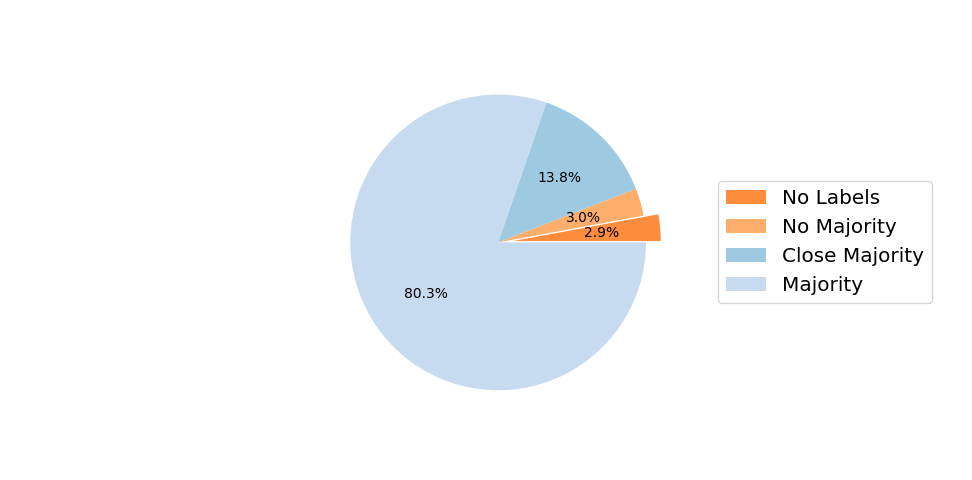
\includegraphics[width=1.0\linewidth]{images/SCARE_label_stats.pdf}
  \end{minipage}
  \stepcounter{myfigure}
  \caption[Accumulated Gains and Losses.]{\textbf{Left}: Number of examples per label after heuristically computing them in the SCARE dataset. {\color{red} WRITE MORE ABOUT IMBALANCE, WHAT TO DO ABOUT IT, COMPUTE F1, ETC} \textbf{Right}: Statistics of label generation. For most of the examples, there was a clear majority decision as to which label should be chosen. \emph{Close Majority} means the majority vote was off by 1. The \emph{No Majority}/\emph{No Labels} portions in the graph were labelled \emph{neutral} by default, while \emph{Clear Majority}/\emph{Close Majority}  were labelled according to the majority vote decision.}
\end{figure}

2.9\% of reviews had no labels at all

3.0\% of votes were non-majority

13.8\% of votes were close (label difference of 1)

\subsubsection{Statistics}

Number of examples: \\
Train: 1,232 \\
Dev: 264 \\
Test: 264

\textbf{merged} \\
average length train: 20.2 (sigma 21.6)

average length dev: 19.2 (sigma 19.1)

average length test: 20.6 (sigma 20.0)

\textbf{subtokenized} \\

average length train: 25.4 (sigma 28.2)

average length dev: 24.0 (sigma 23.1)

average length test: 26.1 (sigma 25.9)

\subsubsection{SOTA}

\cite{sanger2016scare} don't predict a sentiment for each instance, but predict fine-grained
aspect and subjective phrase spans using a CRF-based model.
They report results for exact matches as well as partial matches.
For the aspects, they achieve an F1 score of 69\% and 80\% for subjective phrases, respectively.
Since predicting fine-grained aspect and subjective phrase spans is much more difficult than
etrapolating an overall sentiment of the same utterance, a comparison between the outcomes of the
two tasks are not really comparable.
Furthermore,

\subsection{XNLI}

\cite{conneau2018xnli} built the XNLI corpus by employing professional translators to tranlsate
7,500 English sentence pairs from the Multi-Genre Natural Language Inference (MultiNLI) corpus
\cite{williams2017broad} into fifteen languages.
First, they randomly sample 750 examples from each of the ten text source used in MultiNLI, which
is in English, and then let the same MultiNLI worker pool generate three hypothesis for each
sentence, one for each possible label (\emph{entailment}, \emph{contradicion}, \emph{neutral}).
Each sentence pair was then assigned a gold label that was retrieved by carrying out a majority
vote between the label that was assigned by the person who created the hypothesis and the labels
that were assigend indepentently to the sentence pair by four other people.
Finally, all the sentence pairs were translated into the different languages by tranlators.
In addition, \cite{conneau2018xnli} carry out some tests to verify that the original gold label
still holds in the translated sentences:
They recruited two bilingual annotators to reevaluate 100 examples in English and French, i.e.
they had to re-assign the labels given the sentence pairs.
For tht English examples, the find a 85\% concesus on the gold labels, and for French a
corresponding 83\%, from which they conclude that the overall semantic relationship between the
two languages has been preserved.

% TODO: new stats figure!
%\fig{}{fig:XNLI-stats}{Distribution of labels in the XNLI data set.}{15}{XNLI label statistics}

\begin{examples}
  \label{ex:xnli}
  \item Ich wusste nicht was ich vorhatte oder so, ich musste mich an einen bestimmten Ort in Washington melden.

        Ich war noch nie in Washington, deshalb habe ich mich auf der Suche nach dem Ort verirrt, als ich dahin entsandt wurde.

  \textbf{Neutral}
\end{examples}

\begin{examples}
  \item Natürlich haben sie mich dort gefragt, warum ich ging.

        Sie fragten, warum ich in den Laden ging.

  \textbf{Neutral}
\end{examples}

\begin{examples}
  \item Und ich dachte OK und das war es dann!

        Nachdem ich ja gesagt hatte, endete es.

  \textbf{Entailment}
\end{examples}

\begin{examples}
\item John Burke (Alabama) überprüft und analysiert andere zeitgenössische Konten und findet, dass Boswells nicht nur der genaueste ist, sondern er nutzt es, um Johnsons Charakter zu demonstrieren, wobei andere es lediglich als literarischen Geschwätz abstempeln.

        John Burke ignoriert Aussagen.

  \textbf{Contradiction}
\end{examples}

\begin{examples}
  \item Die öffentliche Bibliothek in Greenlee County, Arizona, zeigt die finanziellen und technologischen Probleme von ländlichen Einrichtungen auf.

        Greenlee County hat eine öffentliche Bibliothek.

  \textbf{Entailment}
\end{examples}


%The label for example \ref{ex:xnli} is \emph{neutral} since the second sentence does not follow necessarily from the first and it also does not contradict it, either.

\subsubsection{Statistics}

Number of Examples: \\
Train: 2,115 \\
Dev: 374 \\
Test: 5,009

\textbf{merged} \\
average length premise train: 20.8 (sigma 9.4) \\
average length hypothesis train: 10.5 (sigma 4.0)

average length premise dev: 20.9 (sigma 9.1) \\
average length hypothesis dev: 11.9 (sigma 4.9)

average length premise test: 21.2 (sigma 9.6) \\
average length hypothesis test: 10.7 (sigma 4.1)


\textbf{subtokenized} \\
average length premise train: 25.8 (sigma 11.9) \\
average length hypothesis train: 12.4 (sigma 4.7)

average length premise dev: 26.3 (sigma 12.1) \\
average length hypothesis dev: 14.3 (sigma 6.0)

average length premise test: 26.1 (sigma 12.0) \\
average length hypothesis test: 12.8 (sigma 5.0)


label distribution:

Neutral: 2,499
Entailment: 2,500
Contradiction: 2,499

% \fig{images/XNLI_premise_subtokenized.pdf}{fig:XNLI-premise-length}{XNLI: Length of subtokenized premises.}{8}{XNLI-Length}
\begin{figure}
  \begin{minipage}{0.45\linewidth}
  \vspace{0pt}
    \includegraphics[width=1.0\linewidth]{images/XNLI_premise_subtokenized.pdf}
  \end{minipage}
  \hfill
  \begin{minipage}{0.45\linewidth}
  \vspace{0pt}
    \includegraphics[width=1.0\linewidth]{images/XNLI_hypo_subtokenized.pdf}
  \end{minipage}
  \stepcounter{myfigure}
  \caption[XNLI Lengths]{\textbf{Left}: Length of subtokenized XNLI premises. \textbf{Right}: Length of subtokenized XNLI hypotheses.}
\end{figure}
In contrary to the above described PAWS-X corpus, there are no identical sentence pairs in XNLI.

\subsubsection{SOTA}

The best system \cite{conneau2018xnli} report for German on their XNLI data set is a model that
relies heavily on translation:
They train their BiLSTM on the MultiNLI data (432,702 instances) and translate the test set of the
given language to English and predict on this data.
Employing this startegy, the authors obtain an accuracy on the German test set of 68.7\%.



\subsection{XQuAD}

``XQuAD consists of a subset of 240 paragraphs and 1190 question-answer pairs from the development
set of SQuAD v1.1 together with their translations into ten languages \textelp{} In order to
facilitate easy annotations of answer spans, we choose the most frequent answer for each question
and mark its beginning and end in the context paragraph using special symbols, instructing
translators to keep these symbols in the relevant positions in their translations''
\cite{artetxe2019cross}.

\begin{examples}
  \label{ex:xquad}
  \item Aristoteles lieferte eine philosophische Diskussion über das Konzept einer Kraft
als integraler Bestandteil der aristotelischen Kosmologie. Nach Ansicht von Aristoteles enthält
die irdische Sphäre vier Elemente, die an verschiedenen „natürlichen Orten“ darin zur Ruhe
kommen. Aristoteles glaubte, dass bewegungslose Objekte auf der Erde, die hauptsächlich aus den
Elementen Erde und Wasser bestehen, an ihrem natürlichen Ort auf dem Boden liegen und dass sie so
bleiben würden, wenn man sie in Ruhe lässt. Er unterschied zwischen der angeborenen Tendenz von
Objekten, ihren „natürlichen Ort“ zu finden (z. B. dass schwere Körper fallen), was eine
„natürliche Bewegung“ darstellt und unnatürlichen oder erzwungenen Bewegungen, die den
fortwährenden Einsatz einer Kraft erfordern. Diese Theorie, die auf der alltäglichen Erfahrung
basiert, wie sich Objekte bewegen, wie z. B. die ständige Anwendung einer Kraft, die erforderlich
ist, um einen Wagen in Bewegung zu halten, hatte konzeptionelle Schwierigkeiten, das Verhalten von
Projektilen, wie beispielsweise den Flug von Pfeilen, zu erklären. Der Ort, an dem der
Bogenschütze den Pfeil bewegt, liegt am Anfang des Fluges und während der Pfeil durch die Luft
gleitet, wirkt keine erkennbare effiziente Ursache darauf ein. Aristoteles war sich dieses
Problems bewusst und vermutete, dass die durch den Flugweg des Projektils verdrängte Luft das
Projektil zu seinem Ziel trägt. Diese Erklärung erfordert ein Kontinuum wie Luft zur
Veränderung des Ortes im Allgemeinen.
\end{examples}

The questions and corresponding answer spans for paragraph \ref{ex:xquad} in the data set are the
following:

\begin{enumerate}
  \item Wer leitete eine philosophische Diskussion über Kraft? $\rightarrow$ Aristoteles
  \item Wovon war das Konzept der Kraft ein integraler Bestandteil? $\rightarrow$ aristotelischen Kosmologie
  \item Aus wie vielen Elementen besteht die irdische Sphäre nach Ansicht des Aristoteles? $\rightarrow$ vier
  \item Wo vermutete Aristoteles den natürlichen Ort für Erd- und Wasserelemente? $\rightarrow$ auf dem Boden
  \item Was bezeichnete Aristoteles als erzwungene Bewegung? $\rightarrow$ unnatürlichen
\end{enumerate}

\cite{artetxe2019cross}

\subsubsection{Statistics}

Number of examples: \\
Train: 820
Dev: 181
Test: 178

\textbf{merged}
average length train answer: 3.3 (sigma 3.2) \\
average length dev answer: 3.4 (sigma 3.4) \\
average length test answer: 3.0 (sigma 3.3)

average length train context: 147.3 (sigma 68.7) \\
average length dev context: 151.7 (sigma 74.1) \\
average length test context: 162.0 (94.8)

average length train question: 11.2 (sigma 3.8) \\
average length dev question: 11.9 (sigma 4.3) \\
average length test question: 11.0 (sigma 4.0)

\textbf{subtokenized}
average length train answer: 5.0 (sigma 4.5) \\
average length dev answer: 5.0 (sigma 4.8) \\
average length test answer: 4.5 (sigma 4.4)

average length train context: 187.9 (85.8) \\
average length dev context: 192.8 (sigma 90.1) \\
average length test context: 205.1 (sigma 113.0)

average length train question: 14.1 (sigma 4.9) \\
average length dev question: 15.3 (sigma 5.3) \\
average length test question: 13.9 (sigma 4.9)

\fig{images/xquad_context_subtokenized.pdf}{fig:xquad-context}{XQuAD: Length of subtokenized Contexts.}{10}{XQuAD-Length}

\subsubsection{SOTA}

Very peculiar architecture that consits in re-training a monolingual English BERT model on
Wikipedia and transfer it to target language following these steps:

\begin{enumerate}
    \item Pre-train a monolingual BERT in English with original pretraining objectives
    \item Transfer model to new language $L_2$, but learn only token embeddings new (transformer body is frozen) with original pretraining objectives
    \item Fine-tune transformer for downstream task in English (transformer body is freezed)
    \item Zero-shot transfer this model to $L_2$ by swapping the English token embeddings with the $L_2$ embeddings
\end{enumerate}

The authors report the following results for the German part of XQuAD:
F1: 73.6
Accuracy (exact match): 57.6\%

\begin{landscape}

\subsection{Overview}

\tab{tab:data-set-overview}{Overview of collected data sets and tasks.}
{\begin{tabular}{l|llll}
  Data Set & NLP Task                   & ML Task                    & \# Examples        & Splits \\
  \hline
  deISEAR  &  Emotion Detection         & Multi-Class Classification & 1,001              & - \\
  MLQA     & Question Answering         & Span Prediction            & 509/4,499          & dev/test \\
  PAWS-X   & Paraphrase Identification  & Binary Classification      & 48,977/1,932/1,967 & train/dev/test \\
  SCARE    & Sentiment Analysis         & Multi-Class Classifiaction & 1,760              & - \\
  %SCARE Rev. &  Sentiment Analysis & Sequence Classification & XYZ & - \\
  XNLI     & Natural Language Inference & Multi-Class Classification &  2,489/7,498       & dev/test \\
  XQuAD    & Question Answering         & Span Prediction            & 1,192              & -
\end{tabular}
}{Overview data sets}


\end{landscape}
% \section{BLEU Scores}
% \label{sec:5_bleuscores}
%
% Table \ref{bleuresults} shows how to use the predefined tab command to have it listed.
% %\tab{#1: label}{#2: long caption}{#3: the table content}{#4: short caption}
% \tab{bleuresults}{BLEU scores of different MT systems}
% {\begin{tabular}{ll|ccc|c}
% language pair  & ABC  & YYY  \\
% \hline
% EN$\rightarrow$DE  & 20.56  & 32.53 \\
% DE$\rightarrow$EN  & 43.35  & 52.53 \\
% \hline
% \end{tabular}
% }{ABC BLEU scores}
%
% And we can reference the large table in the appendix as Table \ref{appendixTable}
%
% \section{Evaluation}
% \label{sec:5_evaluation}
% We saw in section \ref{sec:5_bleuscores}
%
% We will see in subsection \ref{subsec:5_moreeval} some more evaluations.
%
% \subsection{More evaluation}
% \label{subsec:5_moreeval}
%
%
% \section{Citations}
% Although BLEU scores should be taken with caution (see \citet{Callison-Burch2006})
% or if you prefer to cite like this: \citep{Callison-Burch2006} \ldots
%
% to cite: \cite[30-31]{Koehn2005} \\
% to cite within parentheses/brackets: \citep{Koehn2005}, \citep[30-32]{Koehn2005}\\ %\usepackage[square]{natbib} => square brackets
%
% to cite within the text: \citet{Koehn2005}, \citet[37]{Koehn2005}\\
% only the author(s): \citeauthor{Callison-Burch2006}\\
% only the year: \citeyear{Callison-Burch2006}\\
%
% \section{Graphics}
%
% To include a graphic that appears in the list of figures, use the predefined fig command:\\
% %\fig{#1: filename}{#2: label}{#3: long caption}{#4: width}{#5: short caption}
% \fig{images/Rosetta_Stone.jpg}{fig:rosetta}{The Rosetta Stone}{10}{Rosetta}
%
% %\reffig{#1: label}
% And then reference it as \reffig{fig:rosetta} is easy.
%
% \section{Some Linguistics}
%
% (With the package 'covington')\\
%
% Gloss:
%
% \begin{examples}
%  \item \gll The cat sits on the table.
%       die Katze sitzt auf dem Tisch
%   \glt 'Die Katze sitzt auf dem Tisch.'
%     \glend
% \end{examples}
%
% Gloss with morphology:
%
% \begin{examples}
%  \item \gll La gata duerm -e en la cama.
%       Art.Fem.Sg Katze schlaf -3.Sg in Art.Fem.Sg Bett
%   \glt 'Die Katze schl\"aft im Bett.'
%     \glend
% \end{examples}
%
